\documentclass[journal]{IEEEtran}
% useful packages
\usepackage{
                graphicx, setspace, fontspec, caption,
                subcaption, float, polyglossia, rotating,
                lscape, pdflscape, indentfirst, tocloft,
                multirow, mathtools, currfile, xcolor,
				url, chngpage, flexisym, amsfonts, chngpage
            }
% paragraph related package
\usepackage[parfill]{parskip}
% use bzar font(THIS MUST BE LOADED BEFORE XePerian PACKAGE)
\setmainfont{BZar.ttf}
% the dear XePersian package
\usepackage{xepersian}
%
% General settings goes here.
%
% lines space
\renewcommand{\baselinestretch}{1.7}
% paragraph first line indention
\setlength{\parindent}{1cm}
% paragraph spacing
\setlength{\parskip}{1em}
% set graphics' path
\graphicspath{ {images/} }
% make table of content dotted
\renewcommand{\cftsecleader}{\cftdotfill{\cftdotsep}}
% define a new command as {half-space} in english
\newcommand{\halfspace}{\hspace{0pt}}
% define a new command as {half-space} in persian
\newcommand{\نیمفاصله}{\halfspace}
% define a shortcut for half-space in general
\renewcommand{\ }{\halfspace}
% define a new command for ease of use for rendering reference
\newcommand{\renderref}[1] { \begingroup \let\clearpage\relax \include{#1} \endgroup }
% make IEEE sections' counter in arabic format
\def\thetable{\arabic{table}}
\def\thesection{\arabic{section}}
\def\thesubsection{\thesection.\arabic{subsection}}
\def\theparagraph{\thesubsubsection.\arabic{paragraph}}
\def\thesubsubsection{\thesubsection.\arabic{subsubsection}}

\renewcommand\thesectiondis{\arabic{section}}
\renewcommand\thesubsectiondis{\arabic{subsection}.\thesectiondis}
\renewcommand\thesubsubsectiondis{\arabic{subsubsection}.\thesubsectiondis}

\makeatletter
% remove IEEEtran's subsubsection's "," after ":". i.e ":, " -> ": "
\renewcommand{\@IEEEsectpunct}{:\hspace{4pt}}
\makeatother

\newtheorem{definition}{تعریف}[section]

\renewcommand{\یا}{یادگیری\ ارجحیت }
\newcommand{\یم}{یادگیری\ ماشین }
\renewcommand{\تر}{تابع رتبه\ بند }
\newcommand{\ار}{ارجحیت }
\renewcommand{\|}[1][.3em]{\hspace{#1}|\hspace{#1}}
\renewcommand{\,}[1][.3em]{,\hspace{#1}}
\newcommand*{\Scale}[2][4]{\scalebox{#1}{$#2$}}

\DeclarePairedDelimiter\abs{\lvert}{\rvert}
\makeatletter
\let\oldabs\abs
\def\abs{\@ifstar{\oldabs}{\oldabs*}}
\makeatother

\captionsetup{justification=centering}
%
% DOCUMENT BEGIN
%
\begin{document}
\title{ \یا فازی}


\author{
\IEEEauthorblockN{داریوش حسن\ پور آده}\\
\IEEEauthorblockA{
دانشگاه صنعتی اصفهان، دانشکده مهندسی برق و کامپیوتر\\
\emph{{\small \lr{Email: {\tt d.hasanpoor@ec.iut.ac.ir}}}}
}}


%\date{}
\maketitle
\begin{abstract}
\یا یکی از زیررشته\ های \یم می\ باشد که هدف اصلی\ اش یادگیری ارجحیت\ های قابل پیش\ بینی از روی اطلاعات ارجحیت می\ باشد. از نقطه\ نظر یادگیری باناظر \یا روی یک دسته از عناصر که نسبت به یک دسته از برچسب\ ها یا عناصر ارجحیت بیشتری دارند آموزش داده می\ شوند که بتواند در نهایت مدل ارجحیت عناصر دیده نشده را پیش\ بینی کند. \یا فازی ترکیبی از یادگیری ماشین و سیستم\ های فازی می\ باشد که سعی در یادگیری ارجحیت عناصر از طریق یادگیری یک \تر با استفاده از منطق فازی می\ باشد.
\end{abstract}
\textbf{کلمات\ کلیدی}\
\begin{IEEEkeywords}
\textit{\textit{یادگیری ارجحیت، یادگیری ارجحیت فازی، تابع ارجحیت، ‌طبقه\ بندی}}
\end{IEEEkeywords}

\IEEEpeerreviewmaketitle

\قسمت{مقدمه}
یادگیری ارجحیت\زیرنویس{\lr{Preference Learning}} یکی از شاخه\ های یادگیری\ ماشین\زیرنویس{\lr{Machnine Learning}} می\ باشد که در سال\ های اخیر توجه زیادی را به سمت خود جلب کرده است. وظیفه\ ی اصلی یادگیری\ ارجحیت، \emph{یادگیری رتبه\ بندی کردن} عناصر می\ باشد. که با توجه به نوع اطلاعات آموزشی نوع ارجحیت و همچنین نوع رتبه\ بندی می\ تواند تغییر کند. در حالت کلی \یا به استنتاج کردن ارتباطات بین اعضای یک دسته و نگاشت این ارتباطات به مدلی که بتواند ارجحیت نسبی موجود بین اعضای این دسته بخوبی پیش\ بینی کند.\بند
اگر بخواهیم تعریف دقیقی برای \یا ارائه دهیم می\ توانیم بگوییم که \یا به وظیفه\ ی یادگیری پیش\ بینی کردن رابطه\ ی ترتیب\زیرنویس{\lr{Order}} در مجموعه\ ای از اشیا گفت.\
\cite{PL:PL_PEDIA}
\یا از داده\ های اطلاعات ارجحیت\زیرنویس{\lr{Preference Information}} برای اهداف یادگیری خود استفاده می\ کند که این اطلاعات ارجحیت نقش مهمی در تصمیم\ گیری\ های خودکار در زمینه\ های متعددی مانند تئوری تصمیم\ گیری\ های کیفی\
\زیرنویس{\lr{Qualitative decision theory}}،
استدلال غیریکنواخت\
\زیرنویس{\lr{Non-monotonic reasoning}}،
ارضای محدودیت\زیرنویس{\lr{Constraint satisfaction}} و طرح\ ریزی\زیرنویس{\lr{Planning}} و \ldots\hspace{.01em}
 کاربردهای فراوانی دارد. در مرحله\ ی آموزش، الگوریتم\ های \یا به داده\ های ترتیب رتبه\ بندی\زیرنویس{\lr{Ranking Order}} (نیمه)شناخته شده عناصر دسترسی دارند. بسته به مدل و نوع مساله الگوریتم\ های \یا می\ توانند به ۳ دسته\ ی رتبه\ بندی اشیا\زیرنویس{\lr{Object Ranking}}، رتبه\ بندی برچسب\ ها\زیرنویس{\lr{Label Ranking}} و رتبه\ بندی نمونه\ ها\زیرنویس{\lr{Instance Ranking}} تقسیم\ بندی کرد.
\بند در این نوشتار ابتدا مقدمه\ ای بر مفاهیم بنیادی مطرح در \یا آورده شده است و درنهایت با تمرکز بر مقاله اصلی سمینار شرح مفصلی در مورد \یا فازی ارائه خواهیم داد.

\قسمت{\یا}
برای اینکه بتوانیم \emph{\یا فازی} را ارائه دهیم نیاز هست که در این قسمت به معرفی خلاصه\ ای از مفاهیم اولیه و بنیادی زمینه\ ی \یا بپردازیم.

\زیرقسمت{نمادگذاری}
طبق هر شاخه\ ی علمی دیگر به یک سری نماد برای پایه\ گذاری \یا نیاز داریم که در این قسمت به معرفی آن\ ها می\ پردازیم.

\begin{definition}[ارجحیت ضعیف]\label{DEF:WEAK_PREF}
یک ارجحیت ضعیف با نماد $\succeq$ بروی مجموعه\ ای مانند $\mathcal{A}$ یک رابطه\ ی بازتابی و تعددی می\ باشد.
\end{definition}

\begin{definition}[ارجحیت اکید]\label{DEF:STRICT_PREF}
$a \succ b \leftrightarrow (a \succeq b) \wedge (b \not\succeq a)$
\end{definition}

در راستای معناشناسی \یا تعاریف
\ref{DEF:WEAK_PREF} و \ref{DEF:STRICT_PREF}
می\ توان آن\ ها را به صورت جدول
\ref{TAB:NOTATIONS_SEMANTIC}
تعبیر کرد.
\vspace{1.5em}
\begin{table}[H]
    \centering
    \begin{tabular}{c|c}
        \textit{نماد} & \textit{تعبیر} \\\hline\rule{0pt}{1.6em}
        $a \succeq b$ & "جایگزین $a$ حداقل به اندازه\ ی جایگزین $b$ ترجیح داده می\ شود." \\\rule{0pt}{1.6em}
        $a \succ b$ & "جایگزین $a$ بیشتر از جایگزین $b$ ترجیح داده می\ شود."\\
    \end{tabular}
    \caption{تعبیر نمادهای روابط ارجحیت}\label{TAB:NOTATIONS_SEMANTIC}
\end{table}
\vspace{.5em}
\begin{definition}[ترتیب\ اکید کلی\زیرنویس{\lr{Total Strict Order}} -- رتبه\ بندی\زیرنویس{\lr{Order}}]\label{DEF:TOT_STRICT_ORDER}
اگر $\mathcal{A}$ یک مجموعه\ ای از اشیا / جایگزین\ ها\زیرنویس{\lr{Alternatives}} $\{a_1\,\ldots\,a_m\}$ باشد، یک رتبه\ بندی از $\mathcal{A}$ یک جایگشتی همانند $\tau$ از مجموعه\ ی $\{1\,\ldots\,m\}$ می\ باشد بگونه\ ای که $a_i \succ a_j \leftrightarrow \tau(i) < \tau(j)$.
\end{definition}
در تعریف
\ref{DEF:TOT_STRICT_ORDER}
مقدار
$m$
تعداد اشیا/جایگزین\ ها و $a_i$ها همان اشیا/جایگزین\ ها می\ باشند،‌ که از این به بعد به مجموعه\ ی اشیا یا جایگزین\ ها، فقط \emph{جایگزین} گفته خواهد شد. تعریف
\ref{DEF:TOT_STRICT_ORDER}
در واقع فرمت\زیرنویس{\lr{Format}} خروجی کلی الگوریتم\ های \یا را ارائه می\ دهد،‌ به گونه\ ای که خروجی ارجحیت ورودی\ ها یک جایگشتی اندیسی\زیرنویس{\lr{Index Permutation}} ترتیب\ اکید ارجحیت\ های ورودی\ ها می\ باشد بگونه\ ای که \textbf{اندیس} آن جایگزینی که \textbf{دارای ارجحیت بیشتری} نسبت به دیگری است، در مجموعه\ ی $\tau$ \textbf{مقدم\ تر} از دیگری می\ آید.\بند
طبق آنچه که در تعریف
\ref{DEF:TOT_STRICT_ORDER}
آمده، واضح است که الگوریتم\ های \یا درواقع یک جستجوکننده در فضای جایگشتی مجموعه $\tau$ می\ باشد؛ فضای جایگشت\ های $\tau$ را با $\mathcal{S}_m$ نمایش می\ دهند.

\زیرقسمت{انواع الگوریتم\ های رتبه\ بندی}
\label{SUBSEC:TYPES_OF_RANKING_PROBLEMES}
الگوریتم\ های رتبه\ بندی از نظر نوع وظیفه\ ای که به عهده دارند به ۳ تیپ تقسیم\ بندی می\ شوند که عبارتند از رتبه\ بندی برچسب\ ها، رتبه\ بندی اشیا و رتبه\ بندی نمونه\ ها؛ که در این قسمت شرح مختصری از این ۳ تیپ الگوریتم ارائه خواهیم داد.\
\cite{PL:PL_PEDIA}
\زیرزیرقسمت{رتبه\ بندی برچسب\ ها}
در این رتبه\ بندی هدف این است که به ازای یک نمونه برچسب\ ها را براساس ارجحیت مرتب کند. شماتیک ورودی\ ها و خروجی\ ها این نوع الگوریتم در شکل
\ref{FIG:LABEL_RANKING_SCHEMA}
آمده است.
\begin{figure}[H]
    \centering
    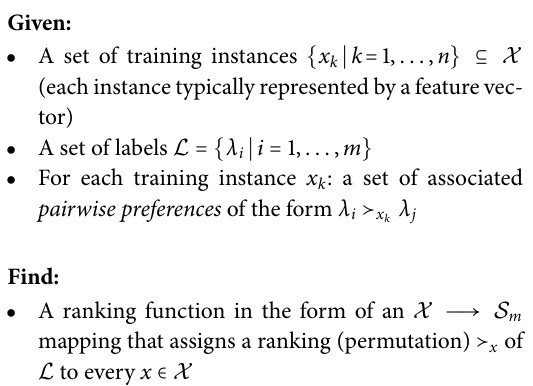
\includegraphics[width=.4\textwidth]{label-ranking}
    \caption{شماتیک کلی الگوریتم\ های رتبه\ بندی برچسب\ ها}\label{FIG:LABEL_RANKING_SCHEMA}
\end{figure}
همانطور که در شکل
\ref{FIG:LABEL_RANKING_SCHEMA}
آمده است الگوریتم\ های رتبه\ بندی برچسب\ ها تعدادی نمونه\ ی آموزشی می\ گیرد که این نمونه\ های آموزشی معمولا به صورت بردار ویژگی\ ها نمایش داده می\ شود. سپس یک سری برچسب و همچنین به ازای هرکدام از نمونه\ ها یک مجموعه\ ی دوبه\ دو مرتب که ارجحیت برچسب\ ها برای هرکدام از نمونه\ ها مشخص شده است را به عنوان ورودی به الگوریتم داده می\ شود.الگوریتم\ های متعلق به رتبه\ بندی برچسب\ ها باید به عنوان خروجی یک \تر است که بتواند به ازای یک شی جایگشت\ های برچسب\ های متعلق به آن شی را با توجه به ارجحیتی که دارند برگرداند.

\زیرزیرقسمت{رتبه\ بندی اشیا}
\label{SEC:OBJECT_RANKING}
در این رتبه\ بندی هدف این است که یک دسته از اشیا را برحسب ارجحیتی که نسبت به هم دارند، را مرتب\ سازی کنیم. که شماتیک ورودی\ ها و خروجی\ ها این نوع الگوریتم در شکل
\ref{FIG:OBJECT_RANKING_SCHEMA}
آمده است.
\begin{figure}[H]
    \centering
    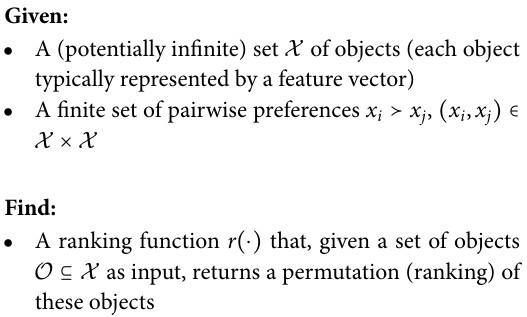
\includegraphics[width=.4\textwidth]{object-ranking}
    \caption{شماتیک کلی الگوریتم\ های رتبه\ بندی اشیا}\label{FIG:OBJECT_RANKING_SCHEMA}
\end{figure}
در شماتیکی که در شکل
\ref{FIG:OBJECT_RANKING_SCHEMA}
آمده است می\ بینیم که همانند رتبه\ بندی برچسب\ ها یک دسته از اشیا را به عنوان ورودی می\ گیرد. سپس یک دسته\ ی (تکه\ ای)مرتب از ارجحیت\ های نسبی این اشیا را نیز به عنوان ورودی به الگوریتم می\ دهیم و نهایت الگوریتم باید یک \تر را بیابد که بتواند ارجحیت\ های هر زیرمجموعه از مجموعه\ ی جهانی اشیا را در قالب یک جایگشتی از اشیا ورودی به عنوان خروجی برگرداند.\بند
توجه شود که مجموعه\ ی (تکه\ ای)مرتب از ارجحیت اشیا که به عنوان داده\ آموزشی به الگوریتم داده می\ شود نیازی ندارد که تمامی ارجحیت\ های موجود میاد اشیا را شامل باشد، به چند دلیل این شرط می\ تواند به قابل پیاده\ سازی بودن الگوریتم کمک زیادی کند. اولین دلیل که بدیهی\ ترین دلیل می\ باشد، این است که ممکن است در کابردهای دنیای واقعی این الگوریتم تمامی \ار های موجود بین اشیا نشاخته نشده باشد. دومین دلیل این است که در صورتی که تمامی \ار های بین اشیا شناخته شده باشد اندازه\ ی مجموعه\ ی مرتب از \ار خیلی بیشتر از تعداد اشیا می\ باشد؛ که از حل
\ref{EQ:OBJECT_RANKING_DATA_OVERLOAD}
می\ بینیم این افزونگی داده\ ای تقریبا $n \over 2$ برابر تعداد اشیا می\ باشد که در کابردهای واقعی این الگوریتم\ ها معمولا تعداد اشیا زیاد است که در نتیجه تعداد ارتباطات مرتب بین آنها بسیار بیشتر از تعداد اشیا می\ باشد که مشکلات خواص خودش را در پی دارد که خارج از حیطه\ ی این نوشتار است.
\begin{equation}\label{EQ:OBJECT_RANKING_DATA_OVERLOAD}
{{n \choose 2} \over n} = {n - 1 \over 2}
\end{equation}
در نتیجه این شرط که الگوریتم\ های رتبه\ بندی اشیا تنها با در اختیار داشتن مجموعه\ ی تکه\ ای مرتب از \ار های میان اشیا باید بتواند مدلی برای رتبه\ بندی اشیا بدست بیاورد؛ باعث می\ شود که این الگوریتم\ های در کاربردهای دنیای واقعی کاربرد پیدا کند.

\زیرزیرقسمت{رتبه\ بندی نمونه}
رتبه\ بندی نمونه همانند رتبه\ بندی اشیا می\ باشد یعنی علاوه بر شماتیک معرقی شده در رتبه\ بندی اشیا ۲ عدد ورودی دیگر را نیز دارد. به این صورت که یک مجموعه اکیدا مرتب(تعریف
\ref{DEF:STRICT_PREF}
را ببینید)
 از برچسب\ ها را نیز اختیار می\ کند که در این مجموعه مرتب از برچسب\ ها آن برچسبی که دارای \ار بیشتری است در ابتدای مجموعه ظاهر شود. و همچنین یک ورودی دیگر نیز به الگوریتم داده می\ شود که مجموعه ارتباطات یک\ به\ یک از هرکدام از اشیا را به برچسب متعلق به آن شی می\ باشد. همچنین در این نوع از الگوریتم\ ها نیازی به مجموعه (تکه\ ای)مرتب از ارجحیت\ های نسبی اشیا به الگوریتم داده شود.

\زیرقسمت{موارد خاص \یا}
همان\ طور که در قسمت
\ref{SUBSEC:TYPES_OF_RANKING_PROBLEMES}
آمده است الگوریتم\ های \یا از نظر اهداف و کاربرد با یک\ دیگر متفاوت هستند، ما همه روزه در میان الگوریتم\ های طبقه\ بندی روزمره\ ای که با آنها سروکار دارم در واقع داریم از الگوریتم\ های \ار استفاده می\ کنیم که در اینجا به معرفی دو نوع از الگوریتم\ های طبقه\ بندی می\ پردازیم که حالت خاصی از الگوریتم\ های \یا می\ باشند.

\زیرزیرقسمت{طبقه\ بندی}
الگوریتم\ های طبقه\ بند\زیرنویس{\lr{Classification}} که همه روزه از آن\ ها استفاده می\ کنیم در واقع حالت خاصی از الگوریتم\ های رتبه\ بندی برچسب\ ها می\ باشد. از آنجایی که در طبقه\ بندی به ازای یک ورودی هدف پیش\ بینی برچسب مرتبط با آن ورودی می\ باشد،‌ می\ توان داده\ ی ورودی را به یکی از الگوریتم\ های \یا(رتبه\ بندی برچسب\ ها) داد سپس از میان مجموعه جایگشت برچسب\ ها که به عنوان خروجی رتبه\ بند برگشت داده خواهد شد، آن برچسبی را که دارای بیشتری \ار است را به عنوان برچسب منتخب برای آن نمونه ورودی انتصاب کرد. به عبارت دیگر می\ توان با استفاده از تعریف
\ref{EQ:PL_USECASE_CLASSIFICATION}
الگوریتم\ های طبقه\ بند را با استفاده از رتبه\ بند برچسب\ های \یا مدل کرد.

\begin{equation}\label{EQ:PL_USECASE_CLASSIFICATION}
\mathcal{C}_{x_k} = \big\{\lambda_i \| \lambda_i \succ_{x_k} \lambda_j \, 1 \leq j \neq i \leq m \big\}
\end{equation}

\زیرزیرقسمت{طبقه\ بندی چند برچسب}
در طبقه\ بندی چند برچسب\زیرنویس{\lr{Multi-label classification}} هر نمونه به یک زیرمجموعه\ ای از برچسب\ ها نسبت داده\ می\ شود. این نوع از الگوریتم\ ها را نیز حالت خاصی از الگوریتم\ های \یا(رتبه\ بندی برچسب\ ها) می\ باشد به\ گونه\ ای که الگوریتم رتبه\ بندی برچسب\ ها یک عدد به عنوان تعداد برچسب\ های نسبت داده شده به اشیا داده می\ شود و الگوریتم بعد از مرتب\ سازی برچسب\ ها بر اساس ارجحیت\ هایی که دارند یک تعداد از برچسب\ ها که دارای ارجحیت بیشتری می\ باشند را به عنوان خروجی بر می\ گرداند. یا یک روش دیگر برای مدل کردن طبقه\ بند چند برچسب با استفاده از رتبه\ بند برچسب\ ها این است که در کنار داده\ های الگوریتم یک حد آستانه مابین $[0\, 1]$ به الگوریتم داده شود و بعد از رتبه\ بندی برچسب\ ها و نرمال\ سازی میزان ارجحیت\ های برجسب\ ها آن برچسب\ هایی که میزان \ار آن\ ها بیشتر از حد آستانه به عنوان خروجی برگشت داده شود. در حالت کلی  می\ توان طبقه\ بند چند برچسب را به صورت تعریف
\ref{EQ:PL_USECASE_MULTI_LABEL_CLASSIFICATION}
با استفاده از رتبه\ بند \ار مدل کرد.

\begin{equation}\label{EQ:PL_USECASE_MULTI_LABEL_CLASSIFICATION}
\mathcal{C}_{x_k} = \big\{\mathcal{L}_k \| \lambda_i \succ_{x_k} \lambda_j \, \lambda_i \in \mathcal{L}_k, \lambda_j \in \mathcal{L}\backslash\mathcal{L}_k\big\}
\end{equation}


\زیرقسمت{انواع روش\ های \یا}
برای \یا دو روش معمول موجود است که یکی بر اساس یادگیری یک تابع سودمندی\زیرنویس{\lr{Learning Utility Functions}} و دیگری یادگیری ارتباطات ارجحیت\زیرنویس{\lr{Learning Preference Relations}} موجود بین داده\ ها را یاد می\ گیرید که برای درک بهتر روش ارائه شده در مقاله اصلی در این بخش به توضیح مختصری نسبت به هریک می\ پردازیم.\بند

\زیرزیرقسمت{يادگیری تابع سودمندی}
یک راه طبیعی برای نشان دادن ارجحیت\ های موجود بین داده\ ها این\ است که جایگزین\ های موجود را با استفاده از یک تابع مطلوبیت ارزیابی کنیم. برای رتبه\ بندی اشیا یک تابع نگاشت
$f : \mathcal{X} \rightarrow \mathcal{U}$
که مقدار سودمندی $f(x)$ به هریک از اشیا $x$ تخصیص می\ دهد را یاد می\ گیریم و درنهایت اشیا را با معیار سودمندی\ ای که از این تابع سودمندی یادگرفته شده محاسبه می\ شود مرتب کرده و به عنوان خروجی برمی\ گردانیم. و در رتبه\ بندی برچسب\ ها به ازای هریک از برچسب\ ها
$\lambda_i\, i = 1\,\ldots\,m$
یک تابع سودمندی
$f_i : \mathcal{X} \rightarrow \mathcal{U}$
یادگرفته می\ شود و در نهایت برچسب\ ها را برحسب مقدار سودمندی\ ای که آن برچسب\ ها دارند مرتب می\ کنیم،
$\lambda_i \succ_x \lambda_j \Rightarrow f_i(x){\geq}f_j(x)$.

\زیرقسمت{یادگیری ارتباطات ارجحیت}
یک روش معمول دیگر در \یا این است که بیاییم و ارتباطات \ار دودویی موجود بین دو اشیا(برچسب) ها را یاد بگیریم. برای رتبه\ بندی اشیا یک تابع \ار دودویی مانند
$\mathcal{Q}(x\, x\textprime)$
یاد می\ گیرد که نشان می\ دهد آیا شی $x$ نسبت به $x\textprime$ \ار دارد یا خیر. در نهایت ترتیب نهایی شامل یک جایگشتی می\ باشد که حداکثر سازگاری را با این ترتیب\ های دودویی داشته باشند. به عبارت دیگر جایگشتی را انتخاب می\ کنیم که مقدار
\ref{EQ:BINARY_OBJECT_RANKING}
را حداکثر کند.
\begin{equation}\label{EQ:BINARY_OBJECT_RANKING}
V_{\mathcal{X}} = \sum_{i = 1} ^ n\sum_{j \neq i = 1} ^ n \mathcal{Q}(x_i, x_j)
\end{equation}
برای رتبه\ بندی برچسب\ ها هم یک روشی به\ نام طبقه\ بندی دوبه\ دو ارائه شده\ است. ایده\ ی این طبقه\ بند دوبه\ دو این است که به ازای هریک از برچسب\ ها یک مدلی مانند
${(\lambda_i\,\lambda_j)\in\mathcal{L}\,1\leq i < j \leq m\,\mathcal{M}_{i,j}}$
را با استفاده از داده\ های آموزشی بدست بیاوریم(یاد بگیریم)؛ در نتیجه به تعداد
${m(m-1)} \over 2$
تعداد مدل نیاز داریم. داده\ های آموزشی شامل اطلاعات ارجحیت برچسب\ ها مانند
$\lambda_i \succ_x \lambda_j$
می\ باشند که به\ صورت مثال\ های آموزشی
$(a\,b)$
تبدیل می\ شوند که برای یادگیری مدل
${b = \max{(i, j)}\, a = \min{(i, j)}\,\mathcal{M}_{a\,b}}$
استفاده می\ شوند. در واقع مدل
$\mathcal{M}_{a, b}$
سعی بر یادگیری مدلی دارد که نگاشت
\ref{EQ:BINARY_LABEL_RANKING_MAB}
را انجام دهد.
\begin{equation}\label{EQ:BINARY_LABEL_RANKING_MAB}
\mathcal{M}_{a, b} \mapsto \begin{cases}
1 & \lambda_a \succ_x \lambda_b\\
0 & \lambda_b \succ_x \lambda_a
\end{cases}
\end{equation}
که این نگاشت می\ تواند توسط یکی از طبقه\ بند کننده\ های دودویی انجام گیرد.


\قسمت{\یا فازی}
مقاله اصلی\
\cite{FPL:MAIN}
\یا را با استفاده از انتگرال چوکت\زیرنویس{\lr{Choquet Integral}} پیاده\ سازی کرده است. که در این قسمت بعد از یادآوری اندازه\ گیری غیرافزایشی\زیرنویس{\lr{Non-additive Measures}} و اینکه چرا انتگرال چوکت می\ تواند برای حل چنین مساله\ ای مفید باشد بحثی خواهیم داشت؛ سپس مروری بر انتگرال چوکت و در انتها روش اصلی ارائه شده در مقاله اصلی را بیان می\ کنیم. نتایج حاصله نیز در بخش بعدی این نوشتار به تفصیل آمده است.

\زیرقسمت{اندازه\ گیری غیرافزایشی}
\label{SEC:NON_ADDITIVE_MEASURE}
برای ارائه\ ی یک دید کاربردی از معنی و مفهوم اندازه\ گیری غیرافزایشی، در این قسمت سعی شده است که این ویژگی را متناسب با کاربردش در \یا با یک مثال فرضی ارائه دهیم.\بند
فرض کنیم که یک مدرسه وجود دارد که به دانش مهندسی دانشجویان\ اش بیشتر از دانش ادبی آن\ ها اهمیت می\ دهد. وهمچنین در سیاست\ های این آموزشکده آمده است که بهتر است دانش\ آموختگانی پروش دهیم که در تمامی علوم آموزش داده\ شده، دارای دانش متعادلی باشند. حال اگر فرض کنیم تنها ۳ درس \emph{ریاضی، فیزیک و ادبیات} در این آموزشکده آموزش داده می\ شود طبق اولین سیاست این آموزشکده که به دانش مهندسی بیشتر از دانش ادبی بها می\ دهد، به نمرات ریاضی و فیزیک دانشجویان وزن بیشتری می\ دهد ولی از طرف دیگر طبق سیاست دوم به دانشجویانی که نمرات متعادل\ تری نسبت به دیگری که واریانس نمرات آن\ ها زیاد است اهمیت نیز می\ دهد.\بند
حال اگر بخواهیم طبق این سیاست\ ها یک اندازه\ گیر تعریف کنیم، مثلا می\ توانیم اندازه\ های زیر را ارائه دهیم که با جزییات مساله سازگارند.
\begin{align*}
&\mu(\{1\,2\,3\}) = 1,&\mu(\{\emptyset\}) = 0\\
&\mu(\{1\}) = \mu(\{2\}) = 0.45,&\mu(\{3\}) = 0.3\\
&\mu(\{1\,3\}) = \mu(\{2\,3\}) = 0.9,&\mu(\{1\,2\}) = 0.5
\end{align*}
که در اینجا طبق آنچه که در اندازه\ گیری\ های بالا مطرح شده است هر یک از دروس ریاضی، فیزیک و ادبیات به تریب با اعداد ۱ و ۲ و ۳ نمایش داده می\ شوند، و می\ توان این تفصیر را کرد که دانشجوی در تمامی دروس خود خوب عمل می\ کند دارای حداکثر درجه\ ی اهمیت یعنی مقدار ۱ برای آموزشکده می\ باشد و دانشجویانی که در هیچ یک از دروس خوب عمل نمی\ کند اهمیتی برای گروه آموزشی آموزشکده ندارند و کسب نمره\ ی خوب در هریک از دروس ریاضی یا فیزیک به تنهایی دارای درجه\ ی اهمیت یکسان ۰.۴۵ می\ باشد این مقدار بیشتر از مقدار درجه\ ی اهمیتی است که برای درس ادبیات گذاشته که مقدار ۰.۳ تخصیص داده شده است می\ باشد. و در انتها دانشجویانی که در کنار یکی از دروس ریاضی یا فیزیک، در درس ادبیات نیز نمره\ ی خوبی کسب کرده\ باشد دارای درجه\ ی اهمیت بیشتری نسبت به دانشجویانی که فقط در درس ریاضی یا فیزیک نمره خوبی کسب کرده\ اند می\ باشد. که در اندازه\ گیری\ های ارائه شده برای این مثال می\ توان ارتباط
\ref{EQ:NON_ADDIVTIVE_MEASURE_EXAMPLE}
را مشاهده می\ کنیم.
\begin{equation}\label{EQ:NON_ADDIVTIVE_MEASURE_EXAMPLE}
\mu(\{1, 2\}) \neq \mu(\{1\}) + \mu(\{2\})
\end{equation}
که رابطه\ ی
\ref{EQ:NON_ADDIVTIVE_MEASURE_EXAMPLE}
در واقع تعریف اندازه\ گیری\ های غیرافزایشی می\ باشد. که در حالت کلی برای اندازه\ گیری\ های که خواص
\ref{EQ:NON_ADDITIVE_MEASURE_1}\ldots\ref{EQ:NON_ADDITIVE_MEASURE_3}
را دارند،‌ اندازه\ گیری\ های غیرافزایشی می\ گویند.
\begin{eqnarray}
\mu(\emptyset) = 0\, \mu(\mathcal{X}) = 1\label{EQ:NON_ADDITIVE_MEASURE_1}\\
\mu(A) \leq \mu(B)\hspace{1.2em}\forall A \subseteq B \subseteq \mathcal{X}\label{EQ:NON_ADDITIVE_MEASURE_2}\\
\mu(\{a_1\,\ldots\,a_k\}) \neq \sum_{i = 1}^{k} \mu(\{a_i\})\label{EQ:NON_ADDITIVE_MEASURE_3}
\end{eqnarray}

یکی از روش\ های مفید ارائه شده برای نمایش اندازه\ گیری\ های غیرافزایشی که در مقاله کمک زیاد برای یادگیری مدل \ار کرده است نگاشت\ موبیوس\زیرنویس{\lr{Mobius Transform}} می\ باشد که به صورت
\ref{EQ:NON_ADDITIVE_MEASURE_MOBIUS_TRANS_1}
\emph{تعریف می\ شود}.
\begin{equation}\label{EQ:NON_ADDITIVE_MEASURE_MOBIUS_TRANS_1}
\mu(\mathcal{B}) = \sum_{A \subseteq \mathcal{B}} m(A)
\end{equation}
به ازای تمامی
$\mathcal{B} \subseteq \mathcal{X}$
که نگاشت\ موبیوس
$m_{\hat{\mu}}$
را که اندازه\ ی
$\hat{\mu}$
به صورت
\ref{EQ:NON_ADDITIVE_MEASURE_MOBIUS_TRANS_2}
تعریف می\ شود.
\begin{equation}\label{EQ:NON_ADDITIVE_MEASURE_MOBIUS_TRANS_2}
m_{\hat{\mu}}(A) = \sum_{v \subseteq A} (-1)^{\abs{A} - \abs{v}}\hat{\mu}(v)
\end{equation}
که در واقع مقدار بدست آمده از
\ref{EQ:NON_ADDITIVE_MEASURE_MOBIUS_TRANS_2}
در واقع می\ توان به عنوان وزن ارزشی\ ای است که اختصاصا به مجموعه\ ی
$A$
داده\ شده است و ارزش ارتباطات غیرمستقیم اجزای تشکیل دهنده\ ی آن مجموعه حذف گردیده\ است.\بند
آنچه که در مثال ابتدای این بخش دیدیم در واقع یک مساله\ ی \یا می\ باشد،‌ که دیدم ارجحیت\ های این مساله یک اندازه\ گیری غیرافزایشی می\ باشد. در اکثر مسائل \یا نوع ارتباطات میان ارجحیت\ ها از نوع اندازه\ گیری\ های غیرافزایشی می\ باشد. به همین علت و طبق آنچه که در مورد انتگرال چوکت مشهور است که به\ خوبی می\ تواند با اندازه\ گیری\ های غیرافزایشی کار کند منطقی به نظر می\ رسد که ترکیب این دو مساله، یعنی \یا و انتگرال چوکت می\ تواند منجر به نتیجه\ ای خوب شود. که همین دلیل انگیزه\ ی اصلی مطرح شده در مقاله نسبت به اینکه چرا از انتگرال\ فازی\ چوکت برای \یا استفاده  شده است.

\زیرقسمت{اهمیت معیارها}
\label{SEC:CRITERIA_IMPORTANCE}
اندازه\ گیری\ های افزایشی را می\ توان به صورت زیر نمایش داد،
\begin{equation*}
\mu(A) = \sum_{x_i \in A} \mu(\{x_i\}) = \sum_{x_i \in A} w_i
\end{equation*}
که اندازه\ ی گیری
$w_i = \mu(\{x_i\})$
وزن معیار\زیرنویس{\lr{Criteria}}
$x_i$
می\ باشد. طبق آنچه که در
\ref{EQ:NON_ADDITIVE_MEASURE_1} و \ref{EQ:NON_ADDITIVE_MEASURE_2}
آمده است این وزن\ ها غیر صفر و
$\sum_{i = 1}^{n} w_i = 1$
می\ باشند. که در اینجا آنچه که واضح است این است که میان معیار\ ها($x_i$ها) هیچ ارتباطی وجود ندارد؛ یعنی اندازه\ گیری روی معیار
$x_i$
مستقل از نتیجه\ ی اندازه\ گیری انجام شده روی معیار
$x_j$
می\ باشد.\بند
حس ضرورت اندازه\ گیری اهمیت معیارها زمانی پدیدار می\ شود که اندازه\ گیری ما از نوع غیرافزایشی باشد. حال فرض کنید یک اندازه\ گیر فازی $\mu$ بروی مجموعه\ ای از معیارها مانند $X$ داده شده است. میزان اهمیت معیار $x_i$ به صورت میانگین میزان افزایش اهمیت با اضافه کرده معیار $x_i$ به یک مجموعه\ ی دیگر مانند
${A \subset X\setminus\{x_i\}}$
که این میانگین\ گیری را می\ توان توسط رابطه\ ی
\ref{EQ:NON_ADDITIVE_MEASURE_IMPORTANCE}
نمایش داد.
\begin{equation}\label{EQ:NON_ADDITIVE_MEASURE_IMPORTANCE}
\varphi(x_i) = {1 \over n}\sum_{A \subset X\setminus\{x_i\}} {1 \over {{n - 1} \choose \abs{A}}}(\mu(A \cup \{x_i\}) - \mu(A))
\end{equation}
که میزان اهمیت معیارها روی یک اندازه\ گیر مانند $\mu$ توسط یک برداری همانند
${\varphi(\mu, X) = <\varphi(x_1)\,\ldots\,\varphi(x_n)>}$
نشان داده\ می\ شود که دارای خواص
\ref{EQ:NON_ADDITIVE_MEASURE_IMPORTANCE_ATTRIB_1} و \ref{EQ:NON_ADDITIVE_MEASURE_IMPORTANCE_ATTRIB_2}
می\ باشد.
\begin{eqnarray}
0 \leq \varphi(x_i) \leq 1\label{EQ:NON_ADDITIVE_MEASURE_IMPORTANCE_ATTRIB_1}\\
\sum_{i = 1} ^ {n} \varphi(x_i) = 1\label{EQ:NON_ADDITIVE_MEASURE_IMPORTANCE_ATTRIB_2}
\end{eqnarray}

\زیرقسمت{انتگرال\ چوکت}
در این قسمت مروری خلاصه بر انتگرال\ چوکت که مورد استفاده در مقاله\ ی اصلی صورت گرفته است، می\ کنیم و سپس با استفاده از نگاشت موبیوس که در بخش
\ref{SEC:NON_ADDITIVE_MEASURE}
تعریف شد تبدیلی رو انتگرال\ چوگت اعمال می\ کنیم که در نهایت مساله\ ی \یا به یک مساله\ ی بهینه\ سازی تبدیل شود\زیرنویس{بنابه اینکه انتگرال\ چوکت جز سرفصل\ های تدریس شده در کلاس بوده و کاملا با مفهوم این انتگرال\ فازی آشنا هستیم از توضیح راجع به جزییات بنیادی این انتگرال خودداری می\ کنم.}.\بند
همان\ طور که می\ دانیم رابطه\ ی انتگرال\ چوکت به صورت
\ref{EQ:CHOQUET_INTEGRAL}
بیان می\ شود\
\cite{COURSE:SAFAYANI}\
.
\begin{align}\label{EQ:CHOQUET_INTEGRAL}
\begin{split}
\mathcal{C}_{\mu}(f) &= \sum_{i = 1} ^ {n} (f(x_{(i)}) - f(x_{(i - 1)})) \cdot \sum_{k = i} ^ {n} \mu(\{x_{(k)}\})\\
&= \sum_{i = 1} ^ {n} (f(x_{(i)}) - f(x_{(i - 1)})) \cdot \mu(A_{(i)})
\end{split}
\end{align}
بگونه\ ای که $(\cdot)$ یک جایگشتی از مجموعه\ ی $\mathcal{S}_m$ است بگونه\ ای که
${0 \leq f(x_{(1)}) \leq f(x_{(2)}) \leq \ldots \leq f(x_{(n)})}$
که
$f(x_{(0)}) = 0$
تعریف شده است و
$A_{(i)} = \{x_{(i)}\,\ldots\,x_{(n)}\}$.\بند
حال اگر بخواهیم انتگرال\ چوکت را از نظر ظاهری با آنچه که برای میزان اهمیت معیارها در بخش
\ref{SEC:CRITERIA_IMPORTANCE}
گفته شد براحتی قابل اثبات است که تابع انتگرال\ چوکت را می\ توان به صورت
\ref{EQ:CHOQUET_INTEGRAL_REWRITE}
بازنویسی کرد.
\begin{align}\label{EQ:CHOQUET_INTEGRAL_REWRITE}
\begin{split}
\mathcal{C}_{\mu}(f) &= \sum_{i = 1} ^ {n} (f(x_{(i)}) - f(x_{(i - 1)})) \cdot \mu(A_{(i)})\\
&= \sum_{i = 1} ^ {n} f(x_{(i)}) \cdot \bigg(\mu(A_{(i)}) - \mu(A_{(i + 1)})\bigg)
\end{split}
\end{align}
حال اگر نگاشت\ موبیوس را بر معادله\ ی بازنویسی شده چوکت در
\ref{EQ:CHOQUET_INTEGRAL_REWRITE}
اعمال کنیم به روابط
\ref{EQ:CHOQUET_INTEGRAL_REWRITE_MOBIUS_TRANS_1}
می\ رسیم.
\begin{align}\label{EQ:CHOQUET_INTEGRAL_REWRITE_MOBIUS_TRANS_1}
\mathcal{C}_{\mu}(f) &= \sum_{i = 1} ^ {n} f(x_{(i)}) \cdot \bigg(\mu(A_{(i)}) - \mu(A_{(i + 1)})\bigg)\\
&\stackrel{\mathclap{\normalfont\mbox{{\tiny MT}}}}{=} \sum_{i = 1}^{n}f(x_{(i)})\cdot\sum_{R \subseteq \mathcal{T}} m(R)\nonumber\\
&= \sum_{T \subseteq \mathcal{X}} m(T) \times \min_{x_i \in T}f(x_i)\nonumber\\
&= \sum_{T \subseteq \mathcal{X}} \sum_{v \subseteq T} (-1)^{\abs{A} - \abs{v}}\mu(v) \times \min_{x_i \in T}f(x_i)\label{EQ:CHOQUET_INTEGRAL_REWRITE_MOBIUS_TRANS_2}\\
\mathcal{T} &= \big\{\mathcal{G} \cup \{x_{(i)}\}\|\mathcal{G} \subset \{x_{(i+1)}\,\ldots\,x_{(n)}\}\big\}
\end{align}
که در
\ref{EQ:CHOQUET_INTEGRAL_REWRITE_MOBIUS_TRANS_2}
تنها چیزی که نامعلوم است مقدار $\mu$ می\ باشد که در بخش بعدی توضیح داده خواهد شد که چگونه یادگرفته خواهد شد و می\ توان به صورت بردار ضرب داخلی
\ref{EQ:CHOQUET_INTEGRAL_INNER_PROD}
نوشت.
\begin{equation}\label{EQ:CHOQUET_INTEGRAL_INNER_PROD}
\bigg\langle m_\varphi\, \varphi(f(x)) \bigg\rangle
\end{equation}
که نگاشت
$\varphi : \mathbb{R}^n \rightarrow \mathbb{R}^{2^n - 1}$
به صورت
\ref{EQ:CHOQUET_INTEGRAL_INNER_PROD_MAPPING}
تعریف می\ کنیم.
\begin{align}\label{EQ:CHOQUET_INTEGRAL_INNER_PROD_MAPPING}
\begin{split}
\varphi(x) &= \varphi(x_1\,\ldots\,x_2)\\
&=\bigg(x_1\,\ldots\,x_n\,\min\{x_1\,x_2\}\,\ldots\,\min\{x_{n-1}\,x_n\}\,\\
&\hspace{1.8em}\min\{x_1\,x_2\,x_3\}\,\ldots\,\min\{x_1\,\ldots\,x_n\}\bigg)
\end{split}
\end{align}
که $m_\varphi$ ماتریس
${\bigg\langle m_1\,\ldots\,m_n\,m_{n+1}\,\ldots\,m_{2^n-1}\bigg\rangle}$
مقادیر بدست آمده توسط نگاشت\ موبیوس می\ باشد که ترتیبش توسط $\varphi(x)$ تعیین می\ شود.

\زیرقسمت{\یا با استفاده از انتگرال\ چوکت}
ایده این مقاله این است که برای رتبه\ بندی اشیا که در بخش
\ref{SEC:OBJECT_RANKING}
معرفی شد، بیاییم \تر را در قالب انتگرال\ چوکت ارائه دهیم. اگر فرض کنیم که هریک از اشیا مانند $o \in \mathcal{O}$ به صورت یک برداری از ویژگی\ ها نمایش دهیم.
\[f_o = \bigg(f_o(x_1)\,\ldots\,f_o(x_n)\bigg)\]
که مقدار
$f_o(x_i)$
مقدار ارزیابی شده شی $o$ براساس معیار $x_i$ می\ باشد. رتبه\ ی شی $o$ را می\ توان با استفاده از انتگرال\ چوکت که در
\ref{EQ:CHOQUET_INTEGRAL_REWRITE_MOBIUS_TRANS_1} و \ref{EQ:CHOQUET_INTEGRAL_REWRITE_MOBIUS_TRANS_2}
معرفی شد به صورت زیر می\ تواند باشد.
\begin{equation}\label{EQ:UTILITY_CHOQUET_INTEGRAL}
U(o) = \mathcal{C}_\mu(f_o)
\end{equation}
حال فرض کنیم داده\ های آموزشی به صورت مجموعه\ ای از اشیا(برداری از ویژگی\ های منتصب به هر شی) به همراه برچسب $l_i$ هر کدام از داده\ ها می\ باشد، $i = 1\,\ldots\,N$. از این داده\ ها یک داده\ ی جدید مانند $\mathcal{D}$ استخراج می\ شود که رابطه\ ی ارجحیت اشیا داخل دیتاست اولیه را به صورت دودویی مدل می\ کند به\ طوری که،
$(o_i\, o_j) \in \mathcal{D}$
که نشان می\ دهد که
$o_i  \succ o_j$
به شرطی که اگر در دیتاست اولیه داشته باشیم
$(o_i\,l_i)$ و $(o_j\,l_j)$
به\ طوری که
$l_i > l_j$.
در راستای ایده\ ی به حداقل رساندن ریسک بصورت تجربی\زیرنویس{\lr{Empirical Risk Minimization}}، مقاله سعی کرده تعداد خطاهای رتبه\ بندی را با استفاده از انتگرال\ چوکت بر روی مجموعه داده\ آموزشی
$\mathcal{D}$
به حداقل برساند.
از آن جایی که انتگرال\ چوکت منحصرا توسط معیار $\mu$ بر روی مجموعه\ ی
$X = \{x_1\,\ldots\,x_n\}$
مشخص می\ شود، بنابراین تعریف مناسب این معیار اهمیت زیادی دارد -- که به همین علت بود که از نگاشت\ موبیوس در
\ref{EQ:CHOQUET_INTEGRAL_REWRITE_MOBIUS_TRANS_1} 
استفاده کرده است.\بند
مقاله با الهام از اصل\ حداکثر\ حاشیه\زیرنویس{\lr{Maximum Margin Principle}} در روش\ های مبتنی بر کرنل\زیرنویس{\lr{Kernel-Based}} یادگیری\ ماشین مساله\ ی یادگیری $\mu$ را به عنوان یک مساله\ ی بهینه\ سازی مدل کرده است.
\begin{equation}
\max_{M\,\xi_1\,\ldots\,\xi_2} \Bigg\{M - {\gamma \over \abs{\mathcal{D}}}\sum_{(o_s\,o_t)\in\mathcal{D}}\xi_s + \xi_t\Bigg\}
\end{equation}
به\ طوری که دارای شروط تعریف شده از
\ref{EQ:LEARNING_MU_COND_FIRST} تا \ref{EQ:LEARNING_MU_COND_LAST}
می\ باشد. که مقدار $M$ نشان دهنده\ ی حاشیه\ ای است که می\ خواهیم حداکثراش کند -- که می\ شود حداقل اختلاف میان میزان سودمندی دو شی که مانند    
$o_s$ و $o_t$
می\ باشد به\ گونه\ ای که
$o_s \succ o_t$.
به\ طور خاص\ تر اگر بخواهییم بگوییم
$M$
یک حاشیه\ ی نرم است که با احتساب این حقیقت که درحالت کلی ارضای تمام نابرابری\ ها به طور هم\ زمان غیرممکن است در نتیجه هر شی
$o_s$
با یک متغییر ضعیف\زیرنویس{\lr{Slack}} همانند
$\xi_s$
در ارتباط است. که این متغییرهای ضعیف نامنفی هستند و مقدار مثبت این متغییر جریمه\ ای متناسب با اندازه خودش تحمیل متحمل می\ شود. و در نهایت
$\gamma$
یک مقدار موازنه\زیرنویس{\lr{Trade-Off}} می\ باشد که هرچقدر مقدارش بیشتر باشد میزان جریمه\ ی تحمیل شده از سوی متغییرهای ضعیف بیشتر می\ باشد.
\begin{align}\label{EQ:LEARNING_MU_COND_FIRST}
&\mathcal{C}_\mu(f_{o_s}) - \mathcal{C}_\mu(f_{o_t}) > M - \xi_s - \xi_t&\forall(o_s\,o_t)\in\mathcal{D}\\
&\xi_s \geq 0\\
&\sum_{T \subseteq X} m(T)= 1\\
&\sum_{B \subseteq A} m(B) \geq 0&\forall A \subseteq X\\
&\sum_{L \subseteq A} m(L) \leq \sum_{K \subseteq B} m(K)&\forall A \subset B \subseteq X\label{EQ:LEARNING_MU_COND_LAST}
\end{align}
بعد از این\ که مقاله با استفاده از معادلات اثبات می\ کند که با استفاده از انتگرال\ چوکت مساله\ ی یادگیری\ ارجحیت\ فازی به یک مساله\ ی بهینه\ سازی تبدیل می\ شود، توضیحی در مورد الگوریتم بهینه\ سازی مورد استفاده در آزمایشات خود نداده است.
\begin{table*}[ht]
    \begin{latin}
    \begin{adjustwidth}{-.in}{0in}
    \centering
    \begin{tabular}{lcccc}
        \hline
        data set & {\#}instances & {\#}attributes & {\#}classes & source\\\hline
        Color(CLR) 1-7 & 120 & 3 & 3 & \cite{DATASET:COLOR}\\
        Scientific Journals(SCJ) & 172 & 5 & 4 & \cite{DATASET:JOURNAL}\\
        CPU & 209 & 6 & 2 & UCI\\
        Auto MPG & 398 & 8 & 6 & UCI\\
        Employee Selection(ESL) & 488 & 4 & 9 & WEKA\\
        Mamographic(MMG) & 830 & 5 & 2 & UCI\\
        Lecture Evaluation(LEV) & 1000 & 4 & 5 & WEKA\\
        Concrete Compressive Strength(CCS) & 1030 & 8 & 6 & UCI\\
        Car Evaluation(CEV) & 1728 & 6 & 4 & UCI\\\hline        
    \end{tabular}
    \end{adjustwidth}
    \end{latin}
    \caption{دیتاست\ ها و ویژگی\ های آن\ ها}\label{TAB:DATASETS_GEN_DESC}
\end{table*}

\قسمت{آزمایشات}
\زیرقسمت{داده\ ها}
در این مقاله ۱۵ عدد دیتاست برای آزمایشات مورد استفاده قرار گرفته\ اند که اکثر آن\ ها از \lr{UCI} و از چارچوب \lr{WEKA} جمع\ آوری شده اند. که همگی آن\ ها معیار\ های سنجش\زیرنویس{\lr{Bench-mark}} برای آزمودن الگوریتم\ های یادگیری می\ باشند. علاوه بر اين\ ها، مقاله تعدادي مجموعه داده از دنياي واقعي، از منابع ديگر مانند داده\ هایی از يک فرآيند پلي\ استر صنعتي رنگرزي و اطلاعات در مورد ارزيابي مجلات رياضي جمع\ آوري کرده است. جدول
\ref{TAB:DATASETS_GEN_DESC}
خلاصه اي از تمام مجموعه\ داده\ ها را نشان مي\ دهد که در سایت نویسندگان\زیرنویس{\lr{http://www.uni-marburg.de/fb12/kebi/research}} مقاله در دسترس عموم گذاشته\ اند.

در ادامه، شرح مختصري در مورد ۲ دیتاست از مجموعه\ داده\ های جدول
\ref{TAB:DATASETS_GEN_DESC}
آورده شده است.\بند
\زیرزیرقسمت{دیتاست \lr{CPU}}
 اين يک مجموعه\ ی داده، معیار سنجش استاندارد از مخزن \lr{UCI} است. که در رابطه با عملکرد نسبی \lr{CPU}های می\ باشد که شامل ۱۰ عدد ويژگي، که سه تا از آن آنجايي که به وضوح فاقد ارزش پيش گويي بوده اند حذف شده\ اند(نام\ فروشنده، نام\ مدل، \lr{EPR}\زیرنویس{\lr{Estimated Relative Performance}}). که مشخصات ویژگی\ های مورد استفاده از این دیتاست در جدول
\ref{TAB:DATASETS_CPU_DESC}
آمده است. در جدول
\ref{TAB:DATASETS_CPU_DATA}
نیز چند سطر از داده\ های این دیتاست آمده است که در این دیتاست برچسب(ویژگی \lr{PRP}) دارای مقداری پیوسته می\ باشد.

\begin{table*}[ht]
    \begin{adjustwidth}{-.in}{0in}
    \centering
    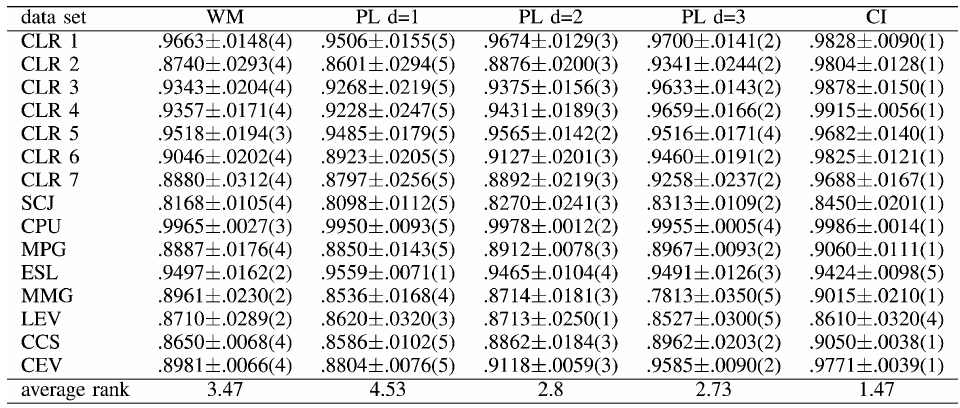
\includegraphics[width=.8\textwidth]{results_1}
    \end{adjustwidth}
    \caption{مقایسه\ ی دقت روش\ های متفاوت با روش
\lr{RankSVM}
با کرنل\ های\\ درجات ۱ تا ۳
و همچنین روش معمول میانگین وزنی    
    }\label{TAB:RESULTS_1}
\end{table*}

\begin{table*}[hb]
    \begin{latin}
    \begin{adjustwidth}{-.in}{0in}
    \centering
    \begin{tabular}{clc}
        \hline
        Feature & Description & Data Type\\\hline
        MYCT   & Machine cycle time in nanoseconds         & Integer\\
        MMIN   & Minimum main memory in kilobytes          & Integer\\
        MMAX   & Maximum main memory in kilobytes          & Integer\\
        CACH   & Cache memory in kilobytes                 & Integer\\
        CHMIN  & Minimum channels in units                 & Integer\\
        CHMAX  & Maximum channels in units                 & Integer\\
        PRP    & Published relative performance(class)     & Integer\\\hline
    \end{tabular}
    \end{adjustwidth}
    \end{latin}
    \caption{ویژگی\ های مورد استفاده\ ی دیتاست \lr{CPU}}\label{TAB:DATASETS_CPU_DESC}
\end{table*}
\begin{table*}[hb]
    \begin{latin}
    \begin{adjustwidth}{-.in}{0in}
    \centering
    \begin{tabular}{cccccccc}
        \hline
        Row\# & MYCT & MMIN & MMAX & CACH & CHMIN & CHMAX & PRP(Class)\\\hline
		1 & 125 & 256  & 6000  & 256 & 16 & 128 & 198\\
		2 & 29  & 8000 & 32000 & 32  & 8  & 32  & 269\\
		3 & 29  & 8000 & 32000 & 32  & 8  & 32  & 220\\
		4 & 29  & 8000 & 32000 & 32  & 8  & 32  & 172\\\hline
    \end{tabular}
    \end{adjustwidth}
    \end{latin}
    \caption{چند مثال از دیتاست \lr{CPU}}\label{TAB:DATASETS_CPU_DATA}
\end{table*}
\زیرزیرقسمت{دیتاست \lr{Mamographic}}
اين مجموعه\ ی داده، دارای اطلاعاتی در مورد سرطان پستان توسط که ماموگرافي بدست آمده است. هدف پيش\ بيني شدت(خوش\ خيم يا بدخيم) توده با استفاده از ويژگي هاي \lr{BI-RADS} می\ باشد. این دیتاست دارای ۶ عدد ویژگی بوده که از این ۶ عدد ویژگی یکی از آن\ ها ویژگی هدف(خوش\ خیم با بدخیم می\ باشد) و یکی از ویژگی\ ها قابل پیش\ بینی نمی\ باشد و دارای ۴ ویژگی دیگر که قابل پیش\ بینی می\ باشند. که مشخصات ویژگی\ های مورد استفاده از این دیتاست در جدول
\ref{TAB:DATASETS_MAMO_DESC}
آمده است. در جدول
\ref{TAB:DATASETS_MAMO_DATA}
نیز چند سطر از داده\ های این دیتاست آمده است.
\begin{table*}[hb]
    \begin{latin}
    \begin{adjustwidth}{-.in}{0in}
    \centering
    \begin{tabular}{clc}
        \hline
        Feature   & Description & Data Type\\\hline
        BI-RADS   & Assessment, (non-predictive!)   & Ordinal\\
        Age       & Patient's age in years          & Integer\\
        Shape     & Mass shape                      & Nominal\\
        Margin    & Mass margin                     & Nominal\\
        Density   & Mass density                    & Ordinal\\
        Severity  & Intensity(class)                & Binominal\\\hline
    \end{tabular}
    \end{adjustwidth}
    \end{latin}
    \caption{ویژگی\ های مورد استفاده\ ی دیتاست \lr{Mamographic}}\label{TAB:DATASETS_MAMO_DESC}
\end{table*}
\begin{table*}[hb]
    \begin{latin}
    \begin{adjustwidth}{-.in}{0in}
    \centering
    \begin{tabular}{ccccccc}
        \hline
        Row\# & BI-RADS & Age & Shape & Margin & Density & Severity(class)\\\hline
        1 & 5 & 67 & 3 & 5 & 3 & 1\\
		2 & 4 & 43 & 1 & 1 & ? & 1\\
		3 & 5 & 58 & 4 & 5 & 3 & 1\\
		4 & 4 & 28 & 1 & 1 & 3 & 0\\
    \end{tabular}
    \end{adjustwidth}
    \end{latin}
    \caption{چند مثال از دیتاست \lr{Mamographic}}\label{TAB:DATASETS_MAMO_DATA}
\end{table*}

\زیرقسمت{مقایسه}
مقاله روش ارائه شده\ ی خود را برای رتبه\ بندی با کرنل\ های خطی و چندجمله\ ای روش \lr{RankSVM} که یکی روش\ های مدرن\زیرنویس{\lr{State of the art}} برای مساله رتبه\ بندی می\ باشد مقایسه کرده است. که نتیجه\ ی این مقایسه\ ها در جدول
\ref{TAB:RESULTS_1}
آمده است. در این جدول که میزان دقت(همراه با انحراف\ معیار چندین اجرا) ۳ الگوریتم میانگین وزنی\زیرنویس{\lr{Weighted Mean}}
و \lr{RankSVM} با ۳ درجه\ ی چندجمله\ ای کرنل و روش ارائه شده در مقاله\
(\lr{CI\footnote{\lr{Choquet Integral}}})
آورده شده است. در کنار هرکدام از دقت\ ها عددی که داخل پرانتز آورده شده است رتبه\ ی دقت الگوریتم مربوطه در آن دیتاست را نمایش می\ دهد و در سطر آخر نیز میانگین رتبه\ ی هرکدام از الگوریتم\ ها آورده شده است. همان\ طور که آورده شده است روش ارائه شده با بیشترین میانگین دقت نتایج مطلوب\ تری را بدست داده است.\بند
برای ملموس\ تر شدن نتایج بدست آمده در جدول
\ref{TAB:RESULTS_1}
جدول
\ref{TAB:RESULTS_2}
را که به\ نوعی ماتریس درهم\ ریختگی رتبه\ ی روش\ ها در اجرا بر روی دیتاست\ های مختلف ارائه شده است که درک بهتری نسبت به اینکه روش ارائه شده در مقاله دیگر روش\ های مدرن در این زمینه را مغلوب کرده است.
\begin{table}[H]
    \centering
    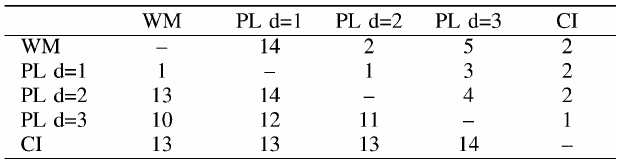
\includegraphics[width=.45\textwidth]{results_2}
    \caption{ماتریس درهم\ ریختگی رتبه\ ی روش\ ها در اجرا بر روی دیتاست\ های مختلف ارائه شده در جدول
    \ref{TAB:DATASETS_GEN_DESC}}\label{TAB:RESULTS_2}
\end{table}
همان\ طور که در جدول
\ref{TAB:RESULTS_2}
مشاهده می\ شود از ۱۵ دیتاست مورد استفاده در آزمایشات مقاله روش ارائه شده دارای بیشترین امتیاز برد نسبت به سایر الگوریتم\ ها مورد مقایسه می\ باشد که الگوریتم\ های مورد مقایسه از روش\ های مدرن در این زمینه می\ باشد.

\قسمت{نتیجه\ گیری}
در این مقاله کاربرد انتگرال چوکت را در مسائل \یا ارائه داده است. درواقع از انتگرال چوکت به عنوان تابع سودمندی برای مسائل رتبه\ بندی استفاده کرده است، که این انتگرال را بخاطر یک سری ویژگی\ های منحصر به فرد انتگرال چوکت که پیشتر آورده شده است انتخاب شده است؛ که مهم\ ترین این ویژگی\ ها این بود که این انتگرال می\ تواند ارتباط وابستگی ارزشی بین معیارها را که به طور ذاتی دارای خاصیت غیر افزایشی می\ باشند، به\ خوبی نشان دهد.\بند
این مقاله نشان داده است که با بکارگیری انتگرال چوکت و نگاشت\ موبیوس مساله\ ی \یا فازی به یک مساله\ ی بهینه\ سازی تبدیل می\ شود که می\ توان با هر الگوریتم بهینه\ سازی اقدام به حل این مساله کرد.\زیرنویس{که البته مقاله در مورد الگوریتم بهینه\ سازی اعمال شده برای مدل ارائه شده در مقاله سخنی نگفته است.} در نهایت با مقایسه\ ای که با مدرن\ ترین الگوریتم\ های موجود در این زمینه نشان داده است که این روش بهتر از بقیه نتیجه داده است.


\begin{thebibliography}{1}
\begin{latin}\scriptsize

\bibitem{FPL:MAIN}
A. F. Tehrani, W. Cheng, and E. Hullermeier, \emph{"Preference Learning Using the Choquet Integral: The Case of Multipartite Ranking"}. in Fuzzy Systems. IEEE Transactions, Dec. 2012, vol. 20, pp. 1102–1113.

\bibitem{PL:PL_PEDIA}
J. Furnkranz and E. Hullermeier, \emph{"Encyclopedia of Machine Learning"}. Springer, 2010, ch. Preference Learning, pp. 789–795.

\bibitem{COURSE:SAFAYANI}
M. Safayani, \emph{"Fuzzy integral lecture"}. In "Fuzzy Set and Systems' Course", Isfahan University Of Technology, Spring 2015.

\bibitem{PL:PL_FRAME}
J. Furnkranz and E. Hullermeier, \emph{"Preference Learning"}. Kunstliche Intelligenz, pp. 60–61, 2005.

\bibitem{DATASET:COLOR}
M. Nasiri and S. Berlik, \emph{"Modeling of polyester dyeing using an evolutionary fuzzy system"}. in Proc. Joint Int. Fuzzy Syst. Assoc. World Congr. Eur. Soc. Fuzzy Logic Technol. Conf., 2009, pp. 1246–1251.

\bibitem{DATASET:JOURNAL}
G. Beliakov and S. James, \emph{"Citation-based journal ranks: The use of fuzzy measures"}. Fuzzy Sets Syst., vol. 167, no. 1, pp. 101–119, 2011.

\end{latin}
\end{thebibliography}
\end{document}
